\indent Old TCPs implementation, would start a connection with the sender injecting multiple segments into the network, up to the window size advertised by the receiver.  This action has no implications if the two host are into the same LAN. While this is OK when the two hosts are on the same LAN; but in the Internet, this schema isn't valid. As is know, between the two end points are routers and getaways, and the flow of packages is not constant, between the two end points some links could be slower than others, and some intermediate buffer's queues could run out of space.\\

The algorithm to starts this ``\textit{clock}'' and to avoid this congestion
 \begin{wrapfigure}{r}{0.5\textwidth}
  \begin{center}
    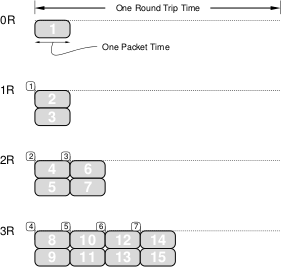
\includegraphics[width=0.48\textwidth]{img/slowstart}
  \end{center}
  \caption{The Chronology of a Slow-Start.\cite{Jacobson:1988:CAC:52325.52356}}
  \label{slowstart}
\end{wrapfigure}
is called \textit{slow start}. It is the responsible to gradually increase the amount of data that is in transit by observing that the a new package is injected into the network until the acknowledgment of a previous packages as arrives from the other end. In other words, it is used to avoid sending more data than the network is capable of transmit.\\

Slow start adds a variable window to the sender's TCP:  the congestion window, called ``\textit{cwnd}'' to the per-connection state.  When a new connection is established or restarting after a loss connection with a host, the congestion window is initialized to one segment, with the size of two times the maximum segment size (MMS)\footnote{The study of MMS is out of the scope of this paper, but more info could be found in \cite{rfc879} and \cite{rfc2460}} .  Each time an ACK is received, the congestion window is increased by one segment (1 MMS).  The sender can transmit up to the minimum of the congestion window and the advertised window.  The congestion window is flow control imposed by the sender, while the advertised window is flow control imposed by the receiver.  The former is based on the sender's assessment of perceived network congestion; the latter is related to the amount of available buffer space at the receiver for this connection.\\

The sender starts by transmitting one segment and waiting for its ACK. When that ACK is received, the congestion window is incremented from one to two, and two segments can be sent.  When each of those two segments is acknowledged, the congestion window is increased to four as seen in figure \ref{slowstart}. Here, the gray numbered boxes are packages and the white are the corresponding ACK. As each ACK arrives, two packages are generated, one for the ACK package that left the ``\textit{pipe}'' and one because an ACK opens the congestion window by one. This provides an exponential growth, it takes time \textbf{$Rlog_2 W$}\cite{Jacobson:1988:CAC:52325.52356}, where R is the round trip time and W is the window size. Although it is not exactly exponential because the receiver may delay its ACKs,typically sending one ACK for every two segments that it receives.\\

At some point the capacity of the internet can be reached, and an intermediate router will start discarding packets.  This tells the sender that its congestion window has gotten too large. Early implementations performed slow start only if the other end was on a different network.  Current implementations always perform slow start.\\
